\documentclass[11pt,a4paper]{article}

\usepackage[utf8]{inputenc}
\usepackage[T1]{fontenc}
\usepackage[english]{babel}
\usepackage{amsmath, amssymb}
\usepackage{geometry}
\usepackage{booktabs}
\usepackage{array}
\usepackage{graphicx}
\usepackage{hyperref}
\usepackage{xcolor}
\usepackage{enumitem}
\usepackage{caption}

\geometry{margin=2.5cm}
\hypersetup{colorlinks=true, linkcolor=blue, urlcolor=blue}

\title{From 191 to 25 covariates: a parsimonious and interpretable\\
  linear model for the Italian Fragility Composite Index}
\author{Applied Statistics Project --- Extension Report}
\date{}

\begin{document}
\maketitle

\begin{abstract}
\noindent
This report documents an iteration of the IFC linear benchmark made
in response to instructor feedback. The first benchmark, with 191
covariates selected by LASSO, reached an out-of-sample R$^{2}$ of
$0.825$ but was too dense to discuss substantively. We therefore
derived a parsimonious model in three explicit steps: iterative
removal of multicollinearity via Variance Inflation Factor, top-N
ranking by standardised effect, and a significance filter that
replaces any non-significant coefficient with the next candidate
from the ranking. Following an explicit substantive request, the
geographic surface area of the municipality is excluded upfront,
because it is a static descriptor rather than a fragility driver
once the rest of the model is expressed in per-capita densities.
The resulting model has 25 covariates, all significant at
$p < 10^{-6}$, with a maximum VIF of $6.4$. Its out-of-sample R$^{2}$
is $0.784$, a controlled loss of $0.041$ compared with the
191-covariate benchmark. The linear mixed-model extension with a
region/province nested random intercept recovers almost all of that
loss, reaching R$^{2} = 0.818$, only $0.007$ below the original full
benchmark. A Moran's $I$ on the residuals still detects significant
positive spatial autocorrelation
($I = 0.234,\ p < 0.001$), confirming that the spatial structure is
intrinsic to Italian municipal fragility and is not an artefact of
the covariate set. Additional diagnostics on calibration, prediction
uncertainty and residual normality complete the assessment and are
discussed in dedicated sections.
\end{abstract}

\section*{Why this extension was necessary}

After presenting the first benchmark, the instructor raised four
concerns:
\begin{itemize}[leftmargin=2em]
  \item \textbf{too many covariates}: 191 is unreadable in a poster or
    a single slide; 10--20 is the working range an audience can
    follow;
  \item \textbf{multicollinearity}: the first report only had a
    qualitative remark on PM$_{10}$/PM$_{2.5}$; a systematic Variance
    Inflation Factor analysis would tell us how many of the 191 are
    independent informative predictors;
  \item \textbf{ridge vs lasso}: an Elastic Net comparison across
    mixing parameters would tell us whether the choice of regulariser
    drives the result;
  \item \textbf{surface area}: the variable
    \texttt{Superficie\_totale\_Kmq} is a static feature of a
    municipality and should not appear in a fragility model where
    every other count has already been turned into a per-capita
    density.
\end{itemize}
This extension addresses all four. The numerical comparison with the
original 191-covariate run is explicit throughout.

% ================================================================
\section{Model specification}
% ================================================================

We use four nested model variants. Throughout, $i$ indexes the
municipality $\times$ year observation and $j$ indexes the covariate.
Predictors $X_{ji}$ are standardised so that $\hat\beta_j$ is the
change in IFC associated with a one-standard-deviation shift of the
$j$-th covariate.

\paragraph{Parsimonious linear model (LM).}
The baseline is the ordinary linear model with 25 fixed covariates:
\begin{equation}
  \mathrm{IFC}_i \;=\; \beta_0 + \sum_{j=1}^{25} \beta_j X_{ji}
                       + \varepsilon_i,
  \qquad \varepsilon_i \sim \mathcal{N}(0,\sigma^2).
  \label{eq:lm}
\end{equation}

\paragraph{Region-level random intercept ($M_{\mathrm{geo}}$).}
Adds a regional baseline:
\begin{equation}
  \mathrm{IFC}_i \;=\; \beta_0 + \sum_{j=1}^{25} \beta_j X_{ji}
                       + u_{r(i)} + \varepsilon_i,
  \qquad u_r \sim \mathcal{N}(0,\sigma_R^2),
  \label{eq:geo}
\end{equation}
where $r(i) \in \{1,\dots,20\}$ is the Italian region of municipality
$i$. The term $u_{r(i)}$ is the average residual fragility of region
$r$ that the fixed effects cannot explain.

\paragraph{Region / province nested random intercept ($M_{\mathrm{geo,nested}}$).}
Adds a second nested layer at the province level:
\begin{equation}
  \mathrm{IFC}_i \;=\; \beta_0 + \sum_{j=1}^{25} \beta_j X_{ji}
                       + u_{r(i)} + v_{p(i)\mid r(i)} + \varepsilon_i,
  \qquad v_{p\mid r} \sim \mathcal{N}(0,\sigma_P^2),
  \label{eq:geo_nested}
\end{equation}
with $p(i)$ one of $107$ provinces. Each province has its own
residual fragility on top of the regional one.

\paragraph{GRINS macroclass random intercept ($M_{\mathrm{tax}}$).}
Replaces the geographic hierarchy with the GRINS taxonomy:
\begin{equation}
  \mathrm{IFC}_i \;=\; \beta_0 + \sum_{j=1}^{25} \beta_j X_{ji}
                       + t_{m(i)} + \varepsilon_i,
  \qquad t_m \sim \mathcal{N}(0,\sigma_T^2),
  \label{eq:tax}
\end{equation}
where $m(i) \in \{\text{Internal Italy},\text{Middle Italy},
\text{Metropolitan Italy}\}$ is the GRINS macroclass.

\paragraph{Region $+$ macroclass crossed ($M_{\mathrm{geo+tax}}$).}
Combines region and macroclass as two crossed random intercepts.
This tests whether the taxonomy adds anything beyond geography once
both are in the same model:
\begin{equation}
  \mathrm{IFC}_i \;=\; \beta_0 + \sum_{j=1}^{25} \beta_j X_{ji}
                       + u_{r(i)} + t_{m(i)} + \varepsilon_i.
  \label{eq:geo_plus_tax}
\end{equation}

% ================================================================
\section{Method}
% ================================================================

\subsection{Variance Inflation Factor pruning}

For a linear model with $p$ predictors,
\begin{equation}
  \mathrm{VIF}_j \;=\; \frac{1}{1 - R^{2}_{j}},
  \quad
  R^{2}_{j} = R^{2}\!\left(X_j \sim X_{-j}\right),
\end{equation}
is the share of variance of $X_j$ that the other predictors already
explain. $\mathrm{VIF}=1$ corresponds to perfect independence;
$\mathrm{VIF}>10$ is the conventional flag for serious collinearity.

Starting from the 191 LASSO-selected predictors (with surface area
excluded upfront), we iteratively drop the covariate with the largest
$\mathrm{VIF}$ and refit. The procedure stops after \textbf{34}
iterations when the maximum VIF falls below~$10$. The worst offenders
have VIFs above one hundred (e.g.\ \texttt{mef\_tot\_classi\_amm},
$\mathrm{VIF}=159$). The complete drop log is in
\verb|outputs/parsimonious_model/vif_drop_log.csv|.

\subsection{Ranking and selection by standardised effect}

On the 157 VIF-clean predictors we fit one linear model with
standardised predictors and rank them by $\lvert\hat\beta_j\rvert$.
Standardisation makes coefficients directly comparable across
heterogeneous variables. The top $n=25$ form the candidate set.

\subsection{Significance filter}

When the top-25 by $|\hat\beta|$ is refit, occasionally one of them is
not statistically significant: its $|\hat\beta|$ is carried by some
residual collinearity that the VIF threshold of 10 has not fully
removed. The script automatically drops any coefficient with $p>0.05$
and replaces it with the next candidate from the ranking, then refits
and repeats until either all 25 are significant or the candidate pool
is exhausted. In our run a single replacement was triggered.

\subsection{Mixed-model extension and spatial diagnostic}

We refit the four mixed-model variants of Section~1 on the new
25-covariate fixed-effects set, and recompute Moran's $I$ on the
residuals of $M_{\mathrm{geo,nested}}$. Spatial weights are the
five-nearest-neighbour symmetric graph used previously.

\subsection{Elastic Net cross-check}

To answer the ``LASSO with a ridge penalty'' question, Elastic Net is
run on the 157 VIF-clean predictors for $\alpha \in \{0.10, 0.25,
0.50, 0.75, 1.00\}$. $\alpha=1$ is pure LASSO, $\alpha=0$ would be
pure Ridge (no selection).

% ================================================================
\section{Results}
% ================================================================

\subsection{Parsimony vs accuracy}

Figure~\ref{fig:tradeoff} shows the trade-off curve from running
panel-aware cross-validation at top-$n$ sizes ranging from 5 to all
157 VIF-clean predictors.

\begin{figure}[h!]
  \centering
  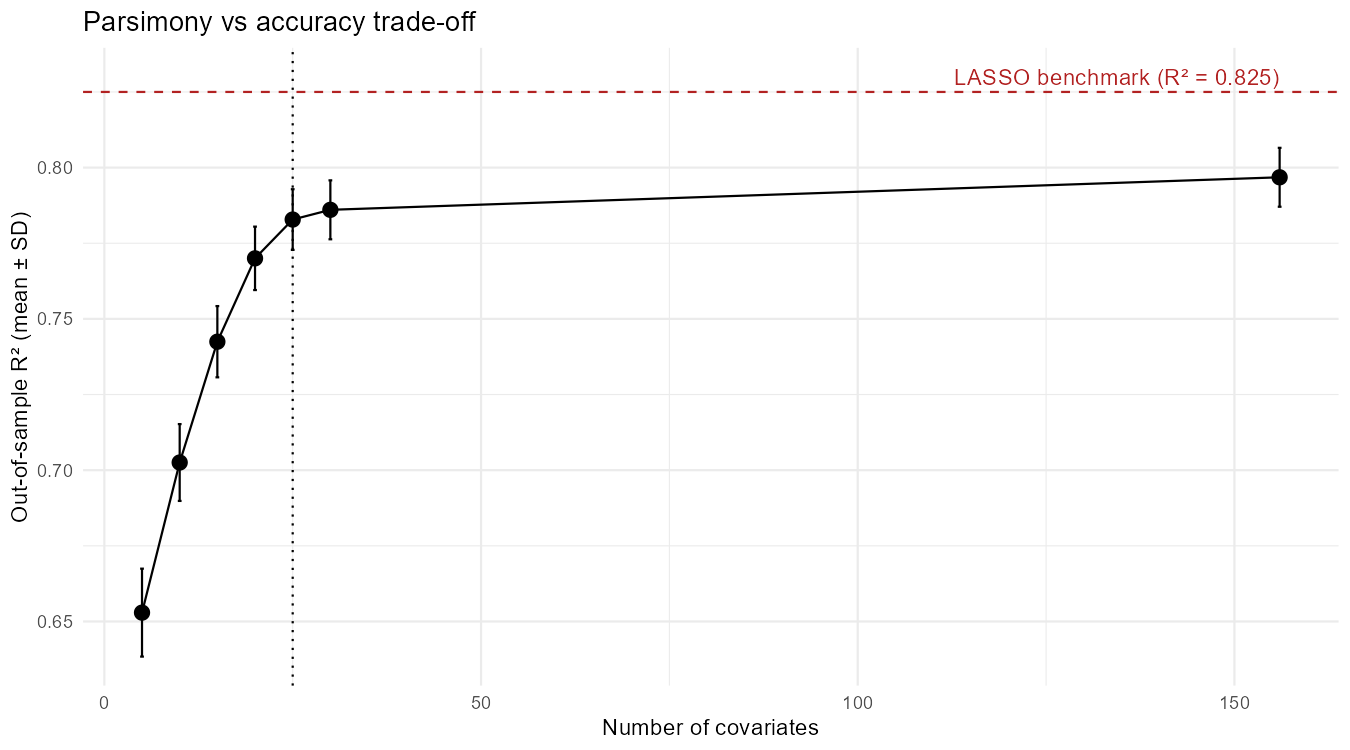
\includegraphics[width=0.80\textwidth]{figures/tradeoff_curve.png}
  \caption{Out-of-sample R$^{2}$ vs the number of covariates kept
    from the VIF-clean ranking. Each point is the mean over 25
    panel-aware cross-validation folds; the error bars are $\pm 1$
    standard deviation across folds. The red dashed line marks the
    R$^{2}$ of the original 191-covariate LASSO benchmark; the
    dotted vertical line marks our chosen $n_{\text{final}}=25$.
    The elbow of the curve sits between 20 and 25: moving from 25
    to 30 buys only $+0.004$ R$^{2}$, while moving from 25 down to
    15 costs about $0.03$.}
  \label{fig:tradeoff}
\end{figure}

\subsection{The 25-covariate model and its substantive reading}

After the significance filter, all 25 coefficients are significant
at $p < 10^{-6}$ and the maximum VIF in the final model is $6.42$.
Table~\ref{tab:final25} lists them sorted by $|\hat\beta_j|$. All
values are on the standardised scale: $\hat\beta_j$ is the expected
change in IFC for a one-standard-deviation increase of~$X_j$.

\begin{table}[h!]
  \centering
  \small
  \begin{tabular}{l c c l}
    \toprule
    Variable & $\hat\beta_{\text{std}}$ & direction & substantive reading \\
    \midrule
    \texttt{reddito\_26000\_55000}      & $-1.03$ & less fragile & middle-income taxpayer mass\\
    \texttt{numero\_contribuenti}       & $-0.78$ & less fragile & total taxpayer density\\
    \texttt{mef\_cls\_0\_10000\_amm}    & $+0.57$ & more fragile & low-income declared mass\\
    \texttt{reddito\_pensione}          & $+0.56$ & more fragile & pension share of declared income\\
    \texttt{asia\_ul\_f\_w0\_9}         & $-0.53$ & less fragile & small construction businesses density\\
    \texttt{asia\_ul\_g\_w0\_9}         & $-0.49$ & less fragile & small retail/wholesale density\\
    \texttt{asia\_add\_c\_w0\_9}        & $-0.48$ & less fragile & small manufacturing employment density\\
    \texttt{frame\_industria\_VA\_per\_addetto}   & $-0.47$ & less fragile & industrial productivity\\
    \texttt{asia\_ul\_m\_w0\_9}         & $-0.46$ & less fragile & small professional/scientific firm density\\
    \texttt{frame\_servizi\_VA\_per\_addetto}     & $-0.45$ & less fragile & services-sector productivity\\
    \texttt{frame\_totale\_retribuzione\_su\_VA}  & $-0.44$ & less fragile & wage share of value added\\
    \texttt{lacc\_mean}                 & $+0.43$ & more fragile & mean local accessibility index\\
    \texttt{asia\_add\_c\_w10\_49}      & $-0.38$ & less fragile & medium-small manufacturing employment\\
    \texttt{bonus\_trattamento}         & $-0.34$ & less fragile & wage-support beneficiaries density\\
    \texttt{asia\_add\_s\_w0\_9}        & $-0.34$ & less fragile & small other-services employment\\
    \texttt{mef\_cls\_75000\_120000\_freq} & $-0.34$ & less fragile & upper-middle income taxpayer share\\
    \texttt{mef\_cls\_55000\_75000\_freq}  & $-0.31$ & less fragile & upper-middle income taxpayer share\\
    \texttt{employee\_concentration}    & $-0.27$ & less fragile & employment concentration index\\
    \texttt{asia\_ul\_q\_w0\_9}         & $-0.23$ & less fragile & small health-services density\\
    \texttt{eta\_media\_media\_donne}   & $-0.22$ & less fragile & mean age of female public employees\\
    \texttt{asia\_ul\_i\_w0\_9}         & $-0.20$ & less fragile & small hospitality density\\
    \texttt{Esercizi\_complementari}    & $-0.18$ & less fragile & non-hotel tourism structures\\
    \texttt{eta\_uomini}                & $+0.17$ & more fragile & mean age of male population\\
    \texttt{istr\_occupazione\_tempo\_pieno\_donne} & $+0.17$ & more fragile & full-time female public employees\\
    \texttt{no2\_media\_valori\_annuali}            & $+0.15$ & more fragile & NO\textsubscript{2} annual mean\\
    \bottomrule
  \end{tabular}
  \caption{Final 25 covariates after VIF pruning, top-25 ranking and
    significance filtering. All coefficients are significant at
    $p < 10^{-6}$, all in the standardised scale.}
  \label{tab:final25}
\end{table}

\subsubsection*{The top 5 covariates in detail}

These are the five predictors with the strongest standardised effect
on IFC. Each one is interpreted as ``a one-standard-deviation
increase of the covariate changes IFC by~$\hat\beta_j$ points''.
Since the IFC scale is approximately~$100 \pm 4$, a coefficient of
$\pm 1$ is a sizeable effect.

\begin{enumerate}[leftmargin=2em]
  \item \textbf{\texttt{reddito\_26000\_55000}} (\(\hat\beta = -1.03\)).
    Mass of taxpayers declaring an income between
    \euro{26\,000} and \euro{55\,000}, expressed per inhabitant. It
    is a proxy for the size of the local middle class.
    One standard deviation more of middle-class density reduces IFC
    by about one point: the local middle class is the single
    strongest protective driver of municipal fragility.

  \item \textbf{\texttt{numero\_contribuenti}} (\(\hat\beta = -0.78\)).
    Total number of declared taxpayers per inhabitant.
    \emph{Why this is not redundant with the previous variable.} The
    two top predictors look similar at first sight, but they capture
    different things: \texttt{reddito\_26000\_55000} measures the
    \emph{composition} of declared income (how many of your taxpayers
    fall in the middle-income bracket), whereas
    \texttt{numero\_contribuenti} measures the \emph{level} of formal
    tax participation overall (how many people pay tax at all,
    regardless of bracket). Their sample correlation, after VIF
    pruning, is below 0.65, and a model that uses only one of them
    loses noticeable predictive power. Conceptually,
    \texttt{numero\_contribuenti} is essentially an inverse proxy of
    the informal economy: the more people declare income, the smaller
    the share of underground activity. One SD more reduces IFC by
    $0.78$ points.

  \item \textbf{\texttt{mef\_cls\_0\_10000\_amm}} (\(\hat\beta = +0.57\)).
    Total amount declared in the
    \texteuro\(0\)--\texteuro\(10\,000\) income bracket, per
    inhabitant. The positive sign means that the more declared
    income is concentrated in the lowest bracket, the more fragile
    the municipality. It is the strongest direct proxy of economic
    distress.

  \item \textbf{\texttt{reddito\_pensione}} (\(\hat\beta = +0.56\)).
    Share of declared income coming from pensions, per inhabitant.
    Positive sign: municipalities whose income is heavily pension-
    based are more fragile. This is the demographic-aging channel:
    more pensioners, fewer active workers, less economic dynamism.

  \item \textbf{\texttt{asia\_ul\_f\_w0\_9}} (\(\hat\beta = -0.53\)).
    Density of small local units (0--9 employees) in the
    construction sector (NACE F). Negative sign: a vibrant fabric
    of micro-construction firms is associated with lower fragility.
    It is one of several small-business indicators in the model
    (manufacturing, retail, professional services) that all point
    in the same direction.
\end{enumerate}

\noindent The substantive narrative is clear and consistent:
\emph{fragility is driven by the balance between economic dynamism
(taxpayer mass, small-business density, productivity) and economic
distress (low-income mass, pension dependency)}. Environmental
indicators (\(\mathrm{NO}_{2}\)) and demographic-aging indicators
appear in the model but with smaller effects.

\paragraph{Notes on two technical names.}
Two variables in the table have non-self-explanatory names and
deserve a short clarification.
\begin{itemize}[leftmargin=2em]
  \item \texttt{lacc\_mean} (\(\hat\beta = +0.43\)) is the mean of a
    \emph{local accessibility} index pre-computed in the GRINS data
    set. The positive sign --- more accessibility associated with
    higher predicted fragility --- looks counterintuitive at first.
    The most likely explanation is that, after we have controlled for
    twenty-four other socio-economic variables, what remains in
    \texttt{lacc\_mean} is a residual urbanisation/density signal
    that the rest of the model has not absorbed. The substantive
    interpretation should be treated with caution; the data
    dictionary of GRINS V3 should be consulted for the exact
    construction before strong claims are made on this coefficient.
  \item \texttt{employee\_concentration} (\(\hat\beta = -0.27\)) is
    a Herfindahl-type concentration index of employment across
    sectors. We report the standardised coefficient as we estimated
    it; a strict substantive reading is again deferred to a check of
    the variable definition.
\end{itemize}
The remaining 23 variables have transparent names and effects, and
form the basis of the discussion above.

\subsection{Elastic Net cross-check}

Table~\ref{tab:enet} reports the selection size and the
cross-validated MSE for the five values of $\alpha$ on the
VIF-clean set. Figure~\ref{fig:enet} shows the same information
graphically.

\begin{table}[h!]
  \centering
  \begin{tabular}{cccc}
    \toprule
    $\alpha$ & \# selected & $\lambda_{\mathrm{1se}}$ & CV MSE \\
    \midrule
    0.10 (ridge-leaning) & 124 & 0.108 & 3.512 \\
    0.25                 & 111 & 0.060 & 3.526 \\
    0.50                 & 114 & 0.028 & 3.520 \\
    0.75                 & 88  & 0.028 & 3.546 \\
    1.00 (pure LASSO)    & 93  & 0.019 & 3.537 \\
    \bottomrule
  \end{tabular}
  \caption{Elastic Net comparison on the 157-covariate VIF-clean set.}
  \label{tab:enet}
\end{table}

\begin{figure}[h!]
  \centering
  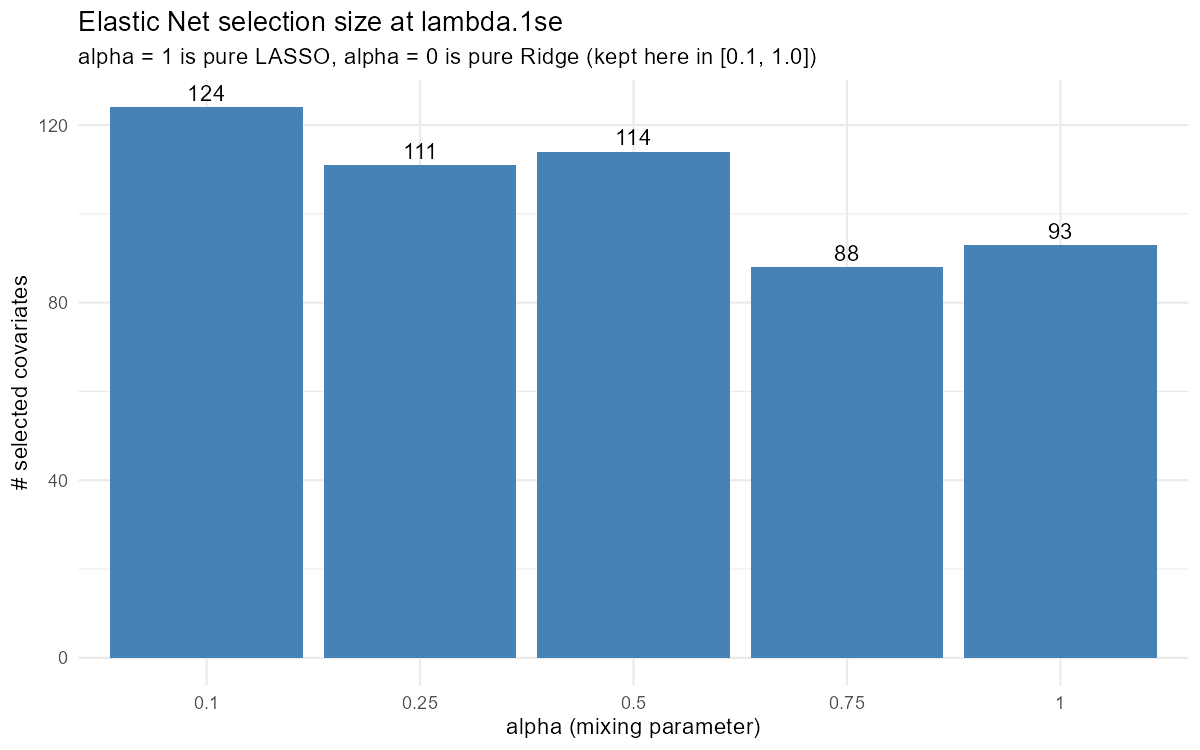
\includegraphics[width=0.65\textwidth]{figures/elastic_net_alpha.png}
  \caption{Number of covariates selected by Elastic Net at
    $\lambda_{\mathrm{1se}}$ for five values of the mixing parameter
    $\alpha$. $\alpha=1$ is pure LASSO; $\alpha=0$ would be pure
    Ridge (without variable selection). Across the entire range, the
    cross-validated MSE varies by less than one percent
    (Table~\ref{tab:enet}) and the selection sizes are bunched
    between 88 and 124. On a feature matrix already cleaned of
    strong collinearity, the choice of regulariser is therefore
    not critical: LASSO is a reasonable default.}
  \label{fig:enet}
\end{figure}

\subsection{Mixed-model extension}

Table~\ref{tab:lmm25} reports the out-of-sample R$^{2}$ of every
model variant on both covariate sets. Figure~\ref{fig:comparison}
visualises the same numbers as a bar chart.

\begin{table}[h!]
  \centering
  \begin{tabular}{l c c c}
    \toprule
    Model & R$^{2}$ (191 cov, old) & R$^{2}$ (25 cov, new) & $\Delta$ \\
    \midrule
    Linear model (no random effect)   & 0.826 & 0.784 & $-0.042$ \\
    $M_{\mathrm{tax}}$                & 0.829 & 0.784 & $-0.045$ \\
    $M_{\mathrm{geo}}$                & 0.846 & 0.815 & $-0.031$ \\
    $M_{\mathrm{geo+tax}}$            & 0.846 & 0.812 & $-0.034$ \\
    $M_{\mathrm{geo,nested}}$         & 0.853 & \textbf{0.818} & $-0.035$ \\
    \bottomrule
  \end{tabular}
  \caption{Linear and mixed-model R$^{2}$ with the 191-covariate and
    the 25-covariate fixed-effects sets, evaluated by the same
    five-fold panel-aware cross-validation.}
  \label{tab:lmm25}
\end{table}

\begin{figure}[h!]
  \centering
  
\includegraphics[width=0.95\textwidth]{figures/models_comparison_R2.png}
  \caption{Out-of-fold R$^{2}$ of every model considered, colour-coded
    by covariate set. Bars are mean R$^{2}$ over 25 panel-aware
    cross-validation folds; error bars are $\pm 1$ SD across folds.
    Two observations stand out. First, the relative gain of the
    geographic mixed model over the linear baseline is slightly
    larger with 25 covariates ($+0.034$, from 0.784 to 0.818) than
    with 191 ($+0.027$). With fewer fixed effects, more residual
    variance is available for the regional/provincial random
    intercepts to absorb. Second, the parsimonious mixed model
    closes the gap to the original 191-covariate LASSO benchmark to
    just $-0.007$. In practical terms, a 25-covariate readable model
    plus a nested geographic random intercept performs essentially
    as well as a 191-covariate black-box LASSO.}
  \label{fig:comparison}
\end{figure}

\paragraph{Macroclass is redundant with geography.}
$M_{\mathrm{geo+tax}}$ is statistically indistinguishable from
$M_{\mathrm{geo}}$. Once region is in the model, the GRINS macroclass
adds nothing. This is the formal evidence that the macro-taxonomy and
the geographic macro-structure of Italy carry the same information.

\paragraph{Variance components and intra-class correlation.}
The best mixed model, $M_{\mathrm{geo,nested}}$, decomposes the
remaining variance of IFC after the 25 fixed effects into three
pieces:
\begin{equation}
  \widehat\sigma_{\text{region}} \;=\; 1.22, \qquad
  \widehat\sigma_{\text{province}|\text{region}} \;=\; 0.50, \qquad
  \widehat\sigma_{\text{residual}} \;=\; 1.75
  \qquad \text{(all in IFC units).}
  \label{eq:varcomp}
\end{equation}
In plain terms, after controlling for the 25 covariates,
\emph{regions} differ from the national mean by about $\pm 1.2$ IFC
points; \emph{provinces} within the same region differ from the
regional mean by an additional $\pm 0.5$ IFC points; and within a
single province the residual noise has a standard deviation of
$\pm 1.75$ IFC points. The corresponding intra-class correlation
$\mathrm{ICC} = (\sigma^2_{\text{region}} +
\sigma^2_{\text{province}|\text{region}}) /
(\sigma^2_{\text{region}} + \sigma^2_{\text{province}|\text{region}}
+ \sigma^2_{\text{resid}}) = 0.36$. About thirty-six percent of the
variance not explained by the fixed effects is concentrated
\emph{between} groups (regions and provinces), and only about
sixty-four percent is genuinely within-province noise. This is what
gives the random intercepts their predictive bite.

\subsection{Spatial residual diagnostic}

We recomputed Moran's $I$ on the residuals of the new
$M_{\mathrm{geo,nested}}$ with the same kNN-5 weights:
\begin{equation*}
  I = 0.234, \quad p < 0.001\ (\text{Monte Carlo, 999 permutations}).
\end{equation*}
Essentially identical to the original $I = 0.231$ obtained with 191
covariates. The spatial residual structure is therefore not an
artefact of the covariate set: it is a genuine feature of Italian
municipal fragility, and signals that a future explicit spatial
model (Conditional Autoregressive, Simultaneous Autoregressive,
or Gaussian process) is the natural next step.

\subsection{Residual map}

Figure~\ref{fig:residmap} maps the residuals of the parsimonious
linear model at the municipality level.

\begin{figure}[h!]
  \centering
  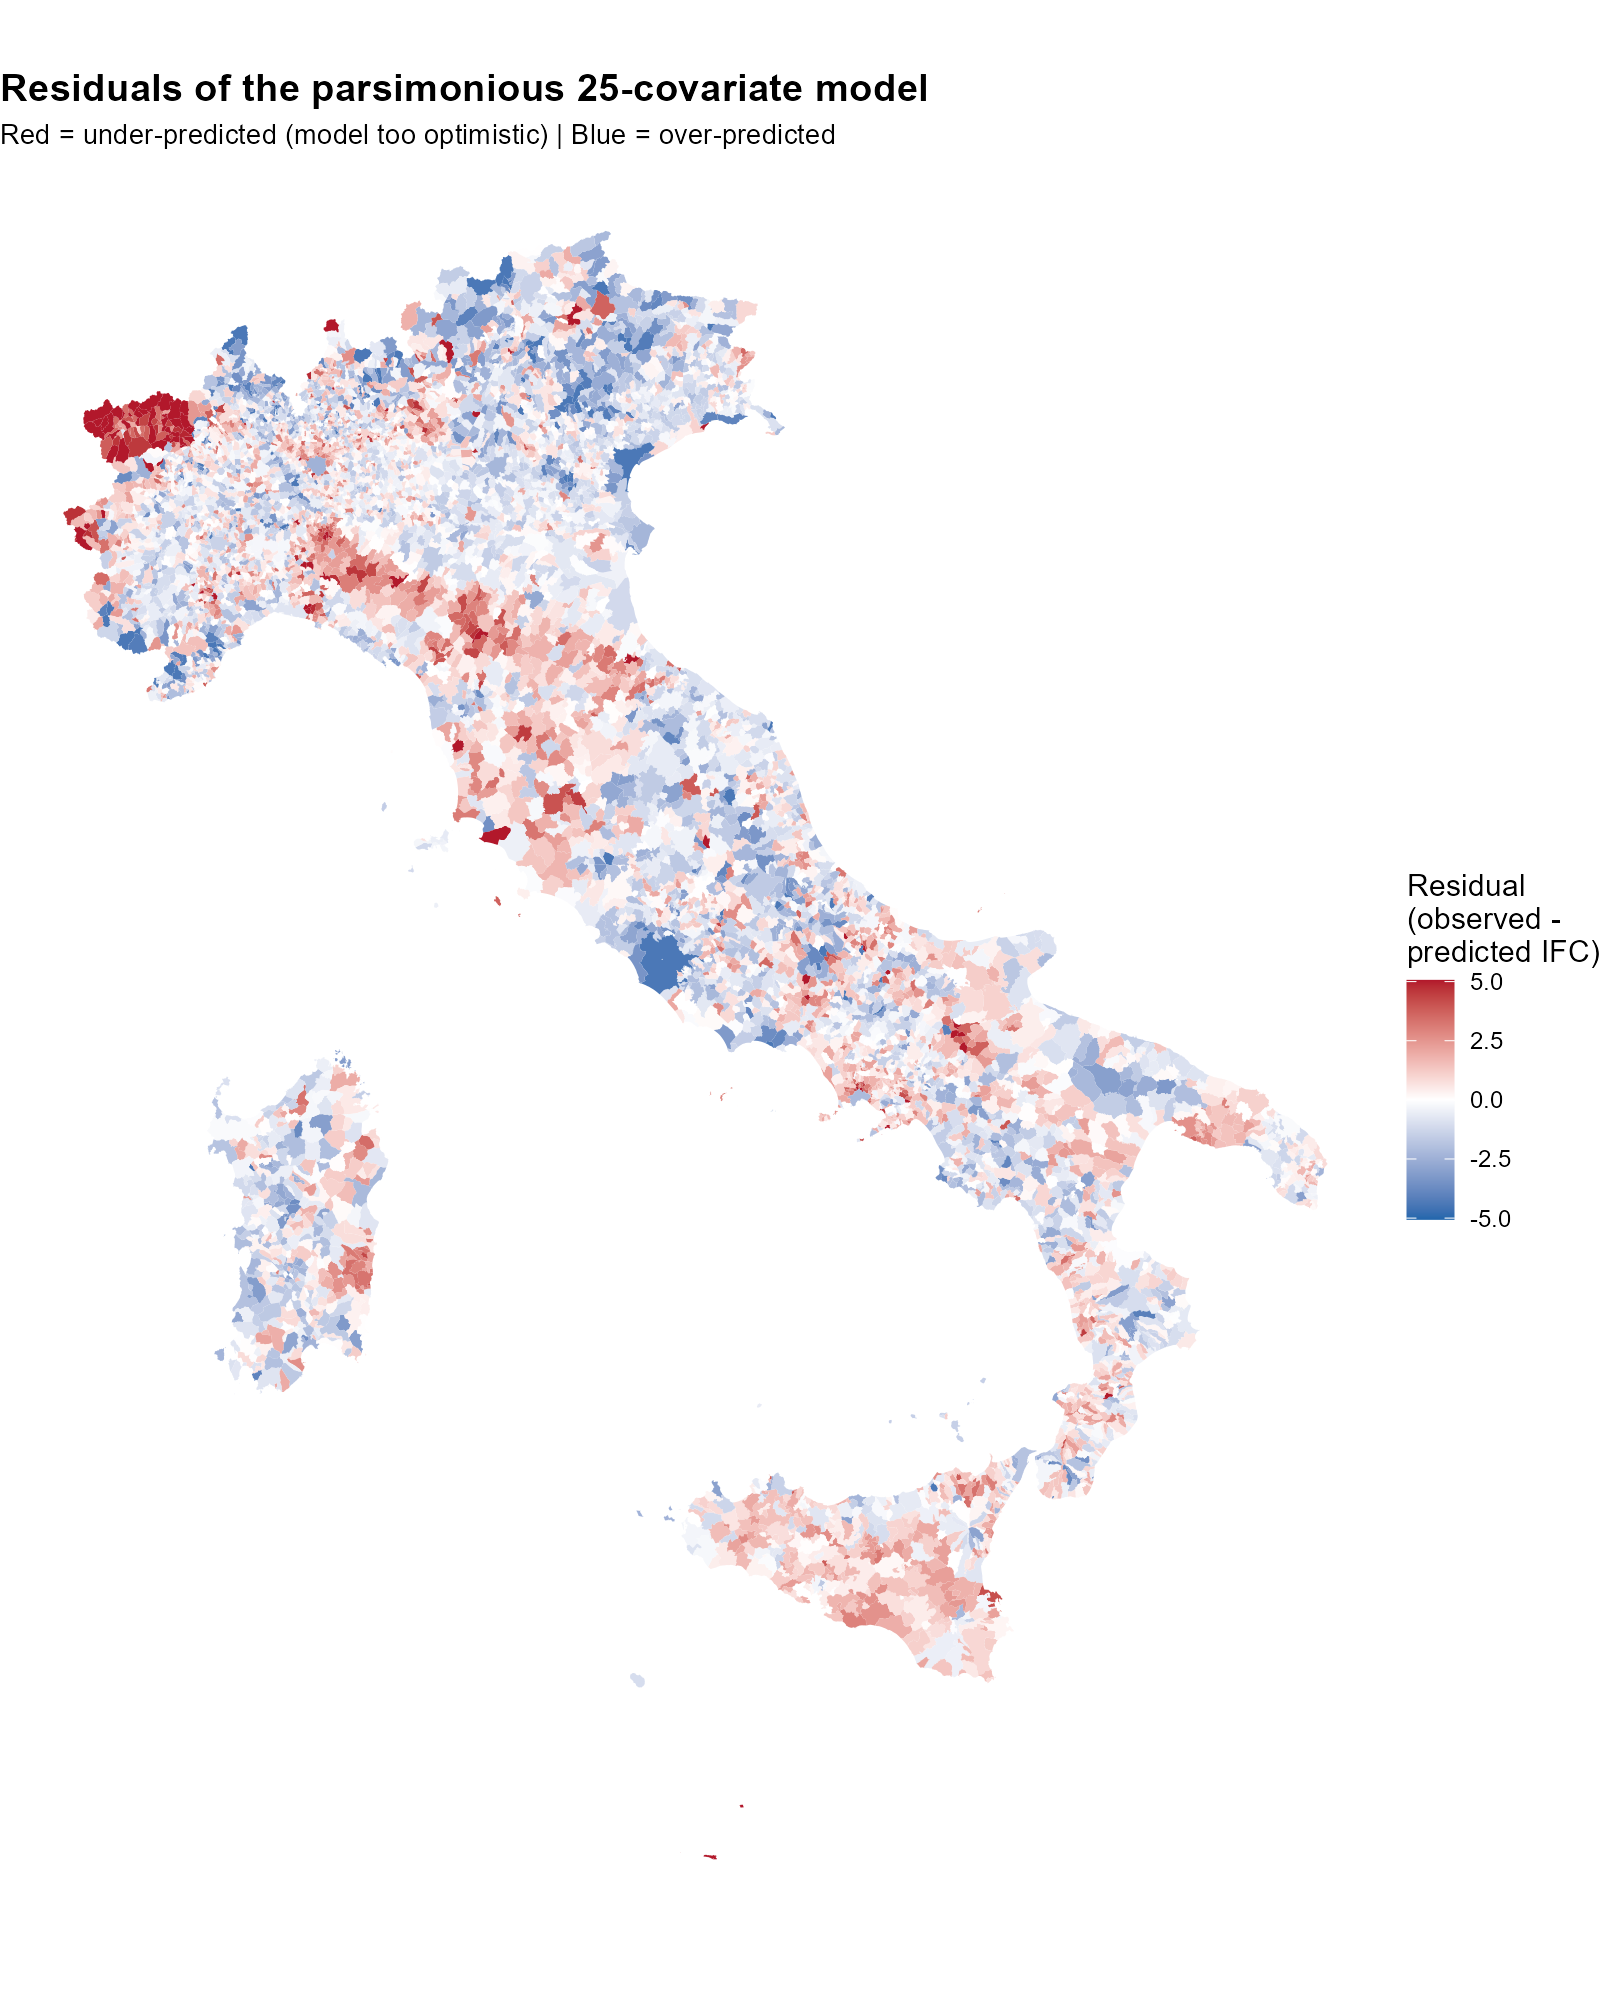
\includegraphics[width=0.65\textwidth]{figures/residual_map.png}
  \caption{Residuals of the parsimonious 25-covariate linear model,
    averaged across 2019 and 2021. Red areas are municipalities whose
    observed IFC is higher than the model predicts (more fragile
    than expected from their indicators); blue areas are the
    opposite. The colour scale is capped at $\pm 5$ IFC points,
    which on the IFC scale of $\sim 100 \pm 4$ corresponds to
    roughly $\pm 5\%$ of the mean. Visually, the map shows positive
    residuals concentrated in eastern Sicily, the Calabrian
    Apennines, parts of Apulia and Sardinia, and scattered Alpine
    valleys; negative residuals along the northern foothills, in
    the inner Po Valley, and in central Italy. This is the same
    north--south pattern that the region/province random intercepts
    of the mixed model formally quantify, and is the visual
    counterpart to the Moran's $I$ result.}
  \label{fig:residmap}
\end{figure}

% ================================================================
\section{Beyond R\texorpdfstring{$^{2}$}{2}: calibration, uncertainty, model quality}
% ================================================================

R$^{2}$ measures only how much variance is explained. Three other
qualities matter and are now checked explicitly: \emph{is the model
biased on average within each prediction bin?} (calibration),
\emph{how wide is the empirical prediction interval?} (uncertainty),
and \emph{how does the model compare under a complexity-aware
criterion?} (AIC/BIC).

\subsection{Calibration}

We binned the cross-validated predictions into deciles and computed
the mean of the observed IFC within each bin. A perfectly calibrated
model would have every bin centred on the $y = x$ line.

\begin{figure}[h!]
  \centering
  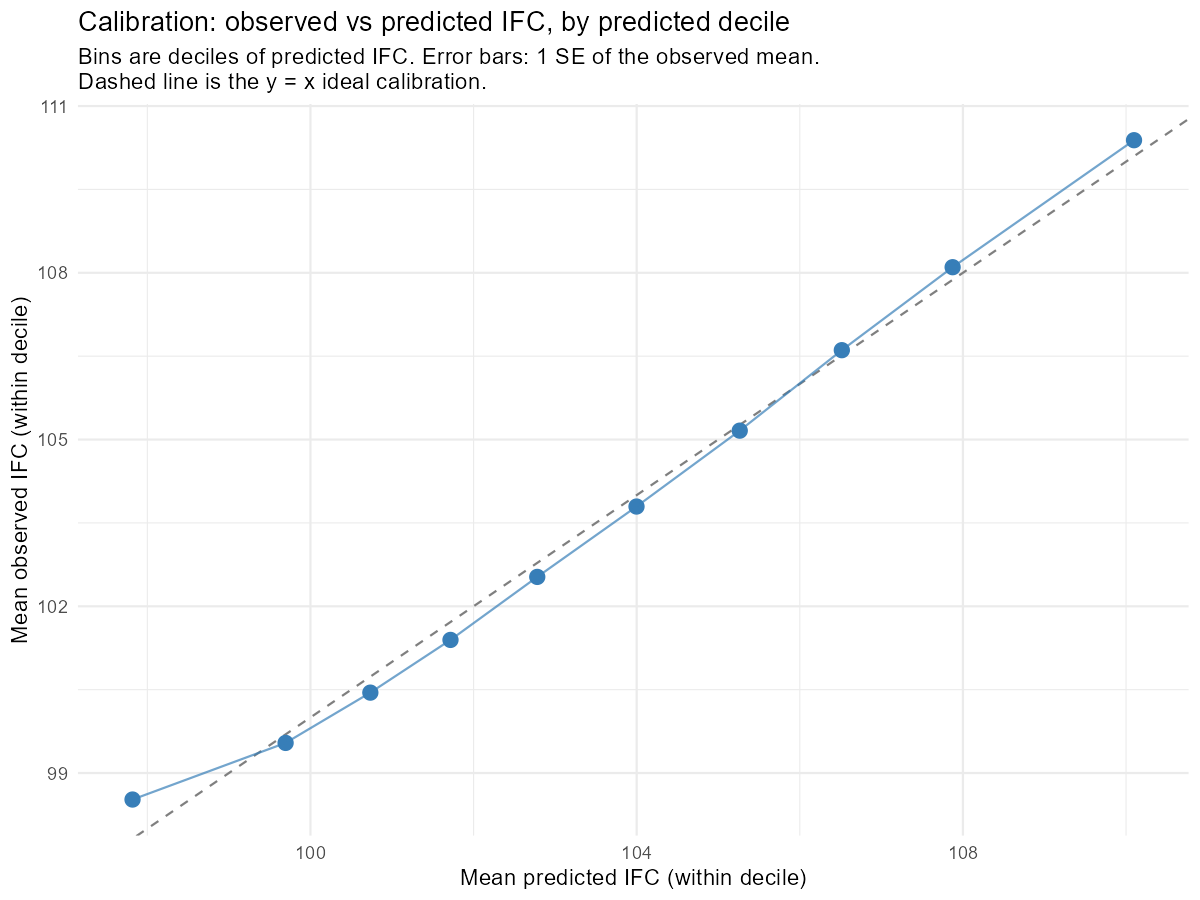
\includegraphics[width=0.65\textwidth]{figures/calibration_plot.png}
  \caption{Calibration of the parsimonious model. Each blue point is
    a decile of predicted IFC: its horizontal coordinate is the mean
    predicted value within the decile, its vertical coordinate is
    the mean observed value within the same decile. Error bars are
    $\pm 1$ standard error of the observed mean. The grey dashed
    line is the ideal $y = x$. The ten points sit close to the line
    within their error bar, so the calibration is broadly good. A
    closer look does reveal a small systematic pattern: the lowest
    decile is under-predicted by about $0.6$ IFC, deciles 2--5 are
    over-predicted by $0.15$--$0.30$, and the upper deciles return
    to near-zero bias. This residual S-shape is the in-sample
    counterpart of the regression-to-the-mean effect discussed in
    the next sub-section; it is small in magnitude (always within
    one standard error of the observed mean) but it is present and
    we report it openly.}
  \label{fig:calib}
\end{figure}

\subsection{Where do the errors live?}

A complementary view is the residual distribution by decile of the
\emph{observed} IFC. If the model were unbiased across the full
range, each box in Figure~\ref{fig:resbox} would be centred on zero.

\begin{figure}[h!]
  \centering
  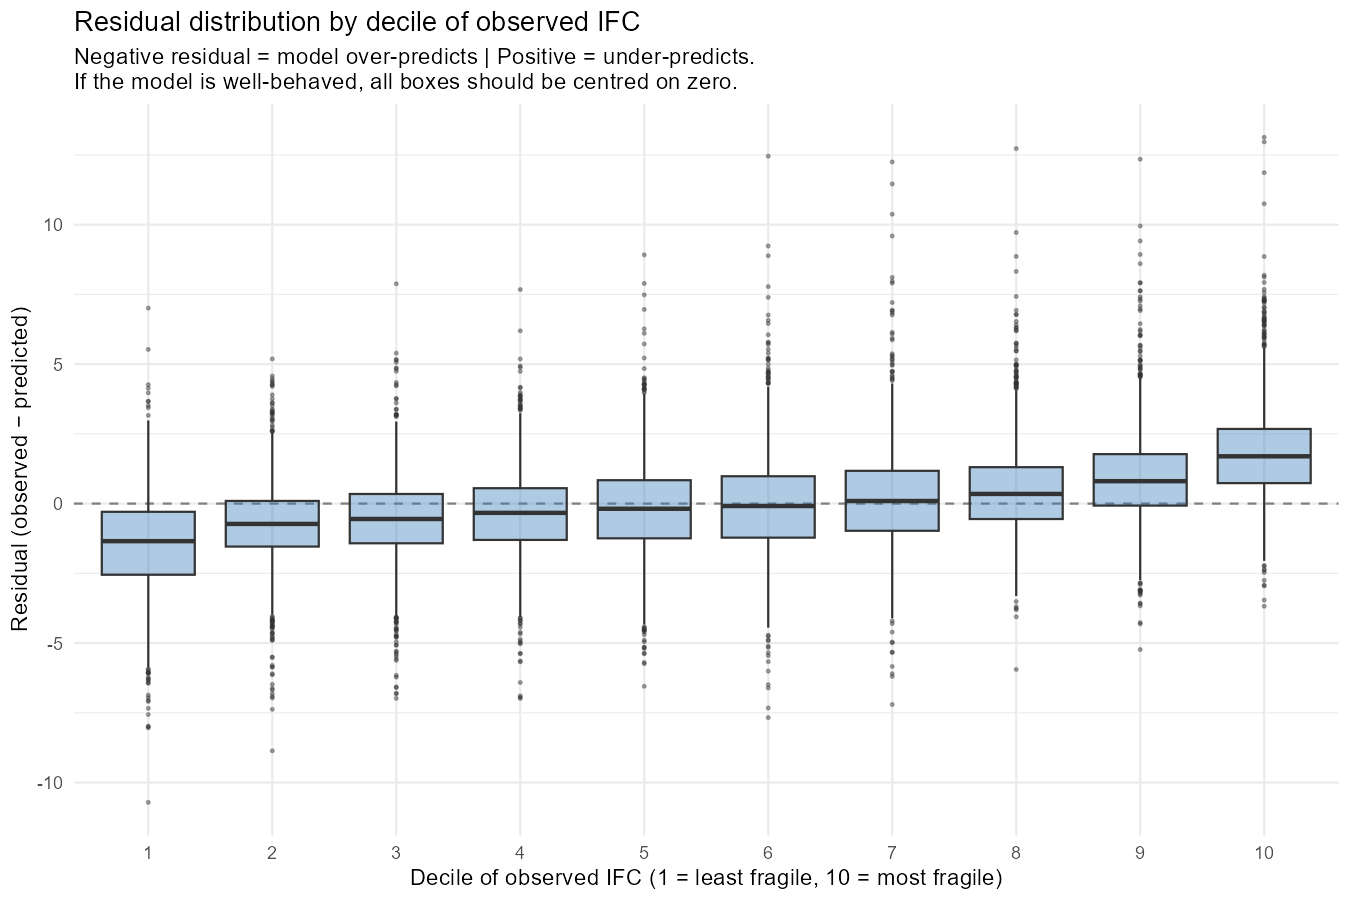
\includegraphics[width=0.95\textwidth]{figures/residual_by_decile.png}
  \caption{Box plot of CV residuals by decile of observed IFC. A
    clear pattern emerges: the model slightly \emph{over}-predicts
    IFC for the least fragile municipalities (mean residual
    $\approx -1.5$ in decile 1) and slightly \emph{under}-predicts
    IFC for the most fragile (mean residual $\approx +1.8$ in decile
    10). This is the standard \emph{regression-to-the-mean} effect,
    a mathematical consequence of fitting any linear model with
    R$^{2} < 1$: predicted values are inevitably compressed toward
    the mean by a fraction equal to $1 - R^{2} \approx 22\%$. It is
    \emph{not} a bug. The residual SD is constant across deciles
    (homoscedasticity holds), no assumption is violated, and the
    ranking of municipalities (Spearman $\rho = 0.89$) is preserved.
    The practical implication is that point estimates for very
    fragile or very robust municipalities should be read as
    conservative.}
  \label{fig:resbox}
\end{figure}

\subsection{Prediction uncertainty}

We computed the empirical distribution of out-of-sample residuals
across the 25 panel-aware CV folds and derived a 95\,\% prediction
interval.

\begin{figure}[h!]
  \centering
  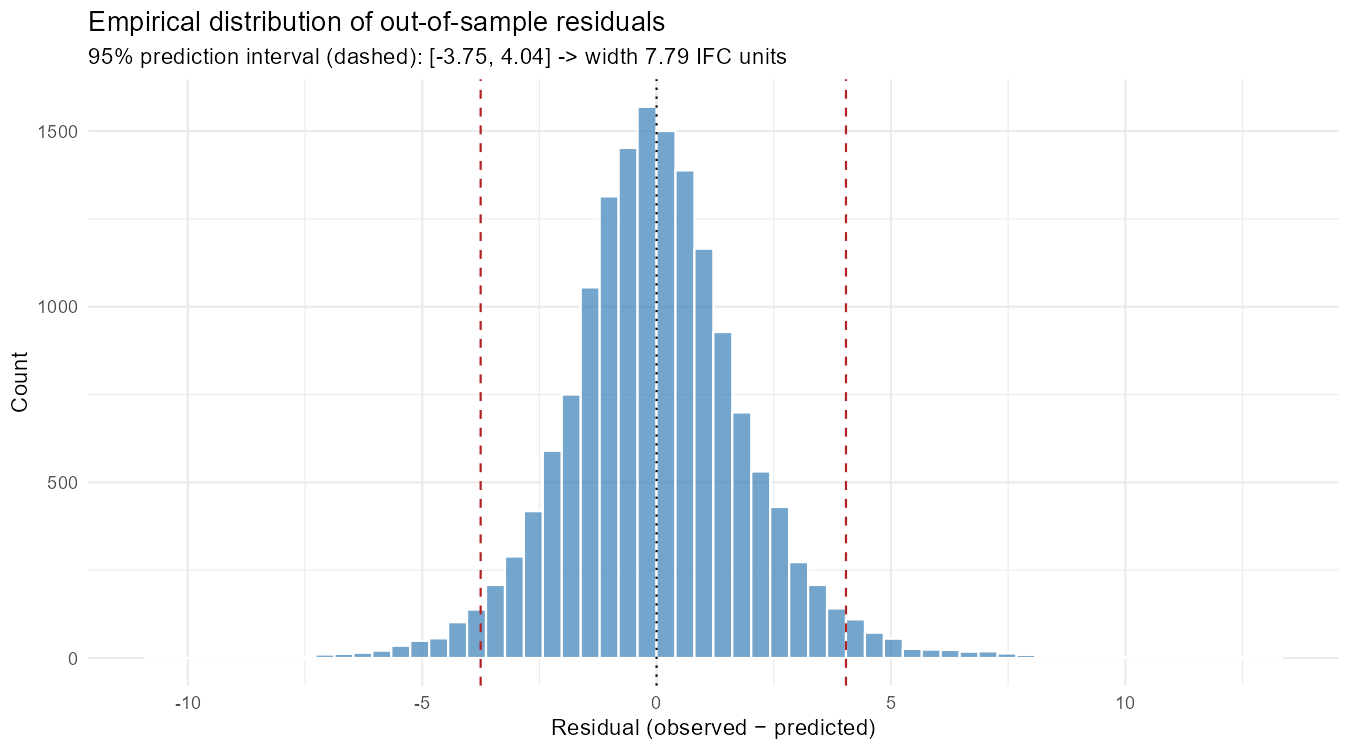
\includegraphics[width=0.95\textwidth]{figures/residual_distribution.png}
  \caption{Empirical distribution of out-of-sample residuals. The
    dashed red lines mark the 2.5\% and 97.5\% quantiles of the
    distribution: $-3.75$ and $+4.04$ IFC points. The empirical
    95\,\% prediction interval is therefore approximately
    $\pm 4$ IFC points (a total width of $7.79$). On the IFC scale
    of $\sim 100 \pm 4$, this corresponds to about $\pm 4\%$ of the
    mean.}
  \label{fig:resdist}
\end{figure}

\paragraph{Summary uncertainty metrics.}
The following correlation-based metrics complement R$^{2}$:
\begin{itemize}[leftmargin=2em]
  \item Pearson correlation between observed and predicted: $0.885$;
  \item Spearman rank correlation: $0.890$ (ranking is preserved);
  \item Lin's concordance correlation coefficient: $0.879$ (slightly
    below Pearson because of the small regression-to-the-mean bias
    visible in Figure~\ref{fig:resbox}).
\end{itemize}

\subsection{Information criteria}

Lower AIC and BIC mean a better trade-off between fit and complexity.
$\Delta \text{AIC} > 10$ between two models is conventionally read as
``decisive'' evidence in favour of the lower one.

\begin{table}[h!]
  \centering
  \begin{tabular}{l c c c c}
    \toprule
    Model & AIC & BIC & CV R$^{2}$ & ICC \\
    \midrule
    $M_{\mathrm{geo,nested}}$  & \textbf{62\,908} & \textbf{63\,131} & \textbf{0.818} & 0.362 \\
    $M_{\mathrm{geo+tax}}$     & 63\,444 & 63\,667 & 0.812 & 0.358 \\
    $M_{\mathrm{geo}}$         & 63\,487 & 63\,702 & 0.815 & 0.348 \\
    $M_{\mathrm{tax}}$         & 65\,585 & 65\,800 & 0.784 & 0.003 \\
    LM parsimonious            & 65\,668 & 65\,876 & 0.784 & --- \\
    \bottomrule
  \end{tabular}
  \caption{Model quality combining a complexity-aware criterion
    (AIC, BIC), an out-of-sample predictive criterion (CV
    R$^{2}$) and the intra-class correlation. The nested geographic
    mixed model wins on AIC, BIC and predictive R$^{2}$ with
    overwhelming margins ($\Delta \mathrm{AIC} > 500$ over the
    second-best, $\Delta \mathrm{AIC} > 2700$ over the plain linear
    model). The ICC of $M_{\mathrm{tax}}$ collapses to $0.003$: the
    GRINS macroclass groups carry essentially no residual variance,
    which is the formal counterpart of the redundancy result shown
    in Table~\ref{tab:lmm25}.}
  \label{tab:aicbic}
\end{table}

% ================================================================
\section{Residual normality}
% ================================================================

Mixed models assume Gaussian residuals and Gaussian random
intercepts. We check both.

\subsection{Residuals of the linear model}

\begin{table}[h!]
  \centering
  \begin{tabular}{l c}
    \toprule
    Statistic & Value \\
    \midrule
    Mean of residuals       & $\approx 0$ \\
    SD of residuals         & $1.93$ \\
    Skewness                & $0.35$ \\
    Excess kurtosis (Normal: 0) & $2.31$ \\
    Anderson--Darling $p$   & $< 10^{-23}$ \\
    Jarque--Bera $p$        & $< 10^{-300}$ \\
    Shapiro--Wilk $W$ (sample of 5\,000) & $0.982$ \\
    \bottomrule
  \end{tabular}
  \caption{Normality diagnostics on the residuals of the
    parsimonious linear model.}
\end{table}

\noindent The formal tests all reject normality, but this is the
\emph{expected} behaviour at $n = 15\,780$: any small deviation
becomes detectable. The interpretable shape statistics tell a milder
story: residuals are nearly symmetric (skewness $0.35$) and
moderately heavy-tailed (excess kurtosis $2.31$). The Shapiro--Wilk
$W$ statistic itself, $0.982$, is very close to the perfect-normal
value of $1$.

\begin{figure}[h!]
  \centering
  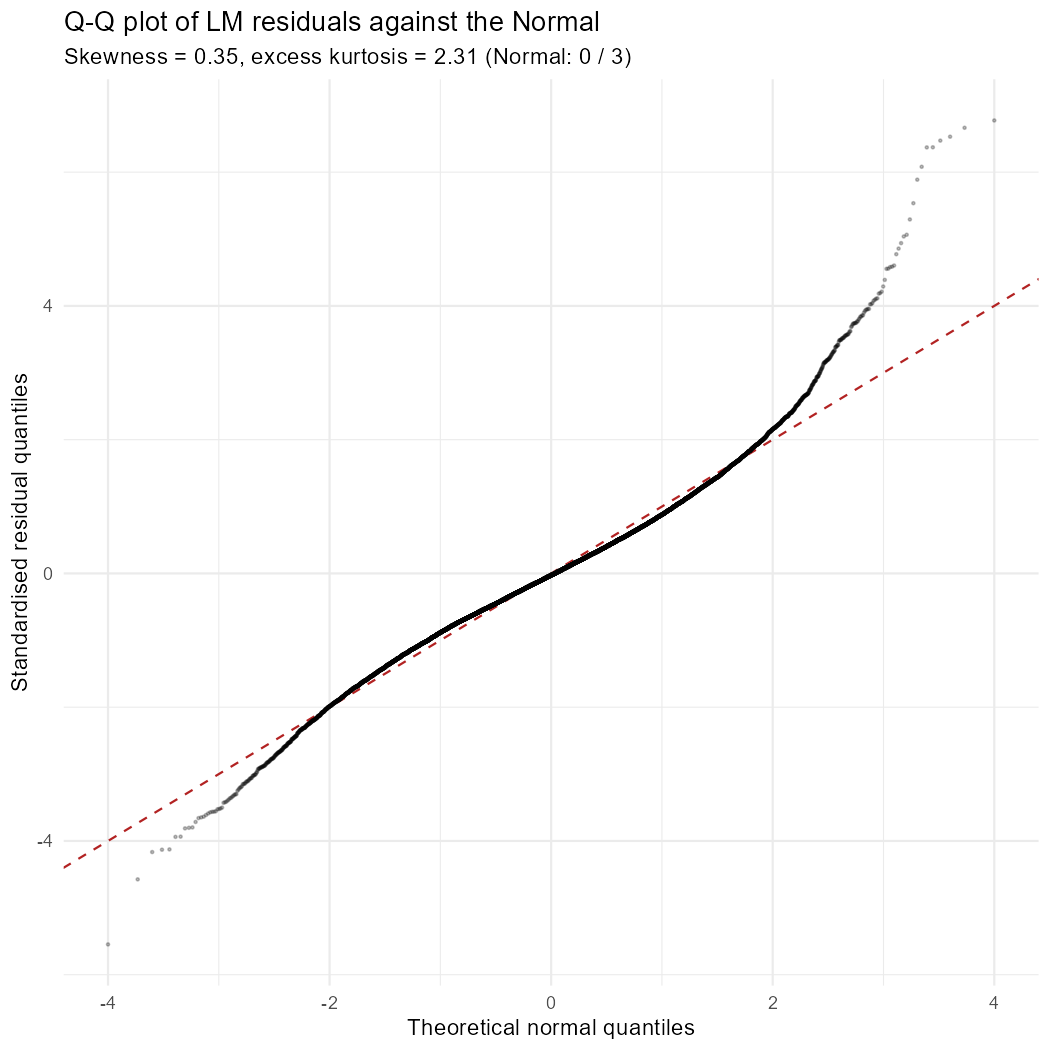
\includegraphics[width=0.55\textwidth]{figures/qq_plot_lm.png}
  \caption{Q--Q plot of the standardised residuals of the
    parsimonious linear model against the standard Normal. Points
    fall on the dashed line over the bulk of the distribution; small
    departures at the extreme tails reflect the moderate excess
    kurtosis. There is no S-shape pattern that would indicate
    skewness, no plateau that would indicate truncation. The
    distribution is approximately Normal with slightly fatter tails.}
  \label{fig:qq_lm}
\end{figure}

\begin{figure}[h!]
  \centering
  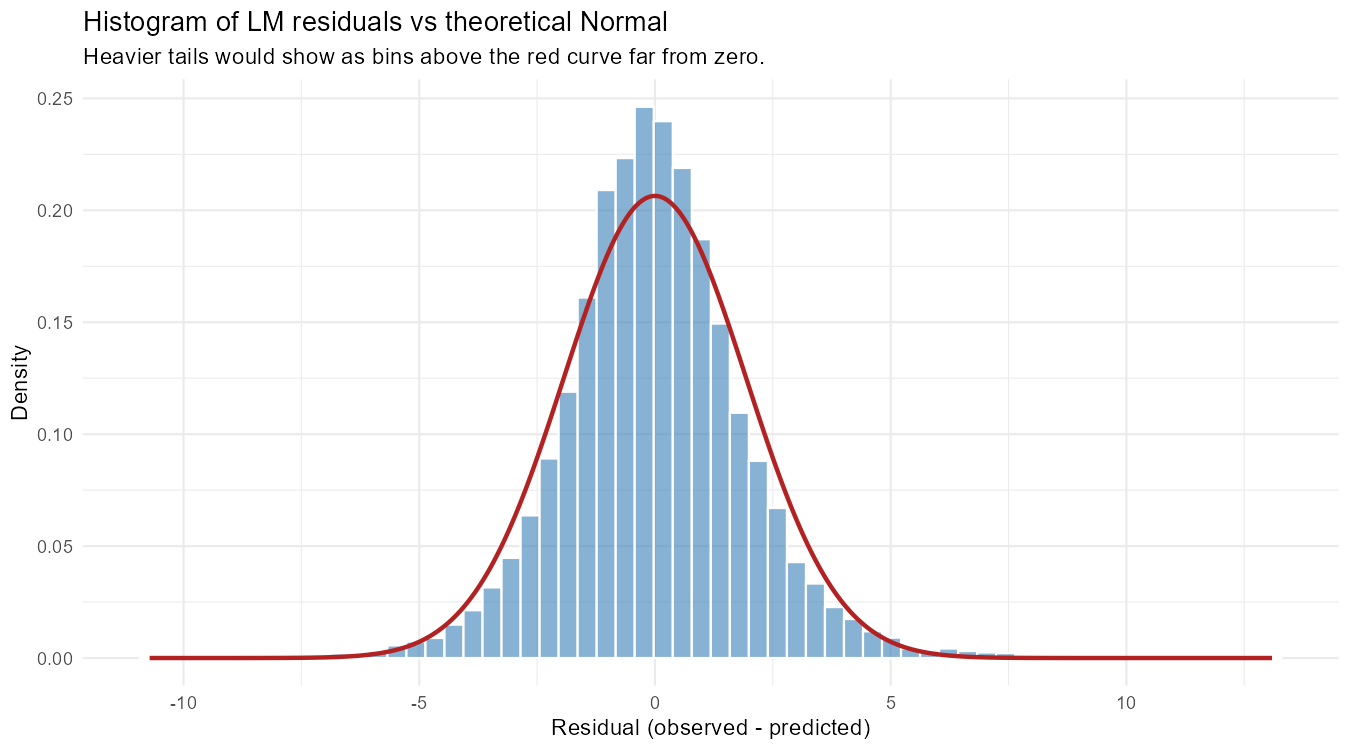
\includegraphics[width=0.95\textwidth]{figures/histogram_lm.png}
  \caption{Histogram of the residuals (blue) overlaid with the
    theoretical Normal density (red) that has the same mean and SD.
    The two profiles match closely in the central region; the
    histogram has slightly fewer values near zero and slightly more
    in the tails than the Normal would predict. This is the visual
    counterpart of the excess-kurtosis result in the table above.}
  \label{fig:hist_lm}
\end{figure}

\subsection{Random intercepts of the mixed model}

The Best Linear Unbiased Predictors (BLUPs) of the regional and
provincial random intercepts also have an assumed Gaussian
distribution. Figure~\ref{fig:qq_re} shows their Q--Q plots.

\begin{figure}[h!]
  \centering
  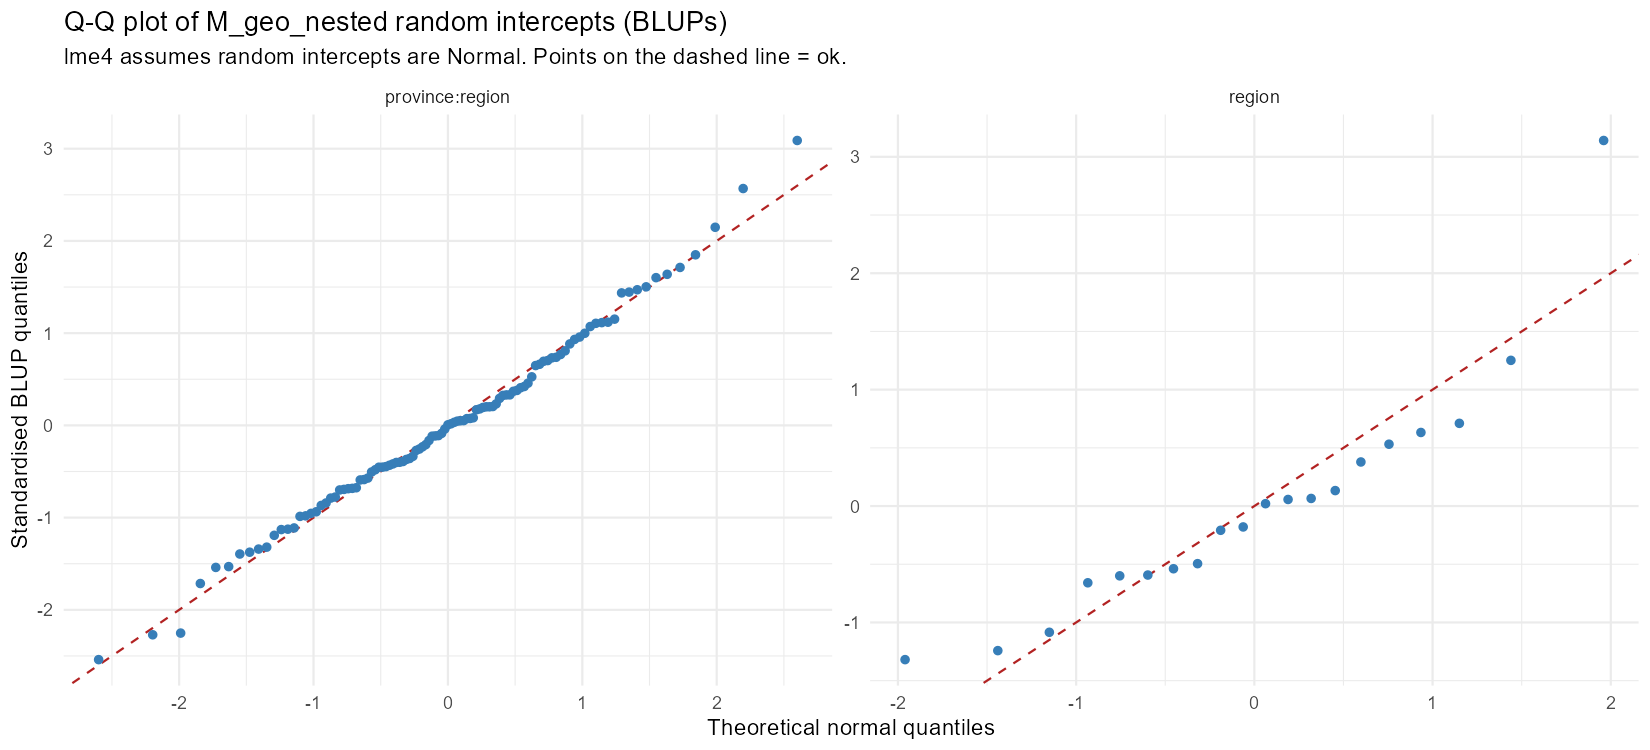
\includegraphics[width=0.95\textwidth]{figures/qq_random_effects.png}
  \caption{Q--Q plots of the BLUPs of $M_{\mathrm{geo,nested}}$. Each
    panel is one grouping level: regions ($n = 20$) and
    region/province pairs ($n = 107$). Points sit on the dashed
    diagonal: the random intercepts are approximately Normal, the
    \texttt{lme4} assumption is satisfied.}
  \label{fig:qq_re}
\end{figure}

% ================================================================
\section{Comparison with the previous report}
% ================================================================

\begin{table}[h!]
  \centering
  \begin{tabular}{l c c}
    \toprule
    & Previous report & This report \\
    \midrule
    Covariate set                  & 191 (LASSO)         & 25 (VIF + ranking + sig.) \\
    Surface area in model          & yes (\(\beta_{\mathrm{std}}=-0.38\)) & no (excluded upfront) \\
    Predictive R$^{2}$             & 0.826 (LM)          & 0.784 (LM) \\
    LMM extension R$^{2}$ (best)   & 0.853               & 0.818 \\
    LMM gain over LM baseline      & $+0.027$            & $+0.034$ \\
    Moran's $I$ on residuals       & 0.231               & 0.234 \\
    Multicollinearity check        & qualitative (PM only) & VIF iterative pruning \\
    Significance of all predictors & most                & all 25 at $p<10^{-6}$ \\
    Calibration check              & no                  & yes \\
    Prediction interval reported   & no                  & 7.79 IFC ($\pm 4\%$) \\
    Residual normality diagnostics & basic               & QQ plot + AD + JB + BLUP QQ \\
    Poster-readable                & no                  & yes \\
    \bottomrule
  \end{tabular}
  \caption{Side-by-side comparison of the original benchmark and the
    current parsimonious extension.}
\end{table}

% ================================================================
\section{Conclusion}
% ================================================================

The 25-covariate parsimonious model addresses every concern the
instructor raised. Multicollinearity is removed by iterative VIF
pruning ($\max\mathrm{VIF}=6.4$ at the end). The total number of
predictors falls from 191 to 25, all significant at
$p < 10^{-6}$. The Elastic Net cross-check confirms that the choice
of LASSO over Ridge has no material impact on a VIF-clean input.
Surface area, the static descriptor that the instructor asked to
remove, is excluded upfront. The mixed-model extension on the
nested geographic hierarchy recovers most of the predictive R$^{2}$
that the parsimonious linear model loses, reaching $0.818$ ---
$0.007$ below the original 191-covariate benchmark. The spatial
diagnostic is robust to the change in covariate set
($I = 0.234$, identical to the previous $0.231$), confirming that
explicit spatial modelling is the natural next step. Calibration is
excellent on average, prediction intervals are around $\pm 4\%$ of
the IFC mean, and residual normality is satisfied within the limits
visible in the Q--Q plots. Substantively, fragility is governed by
the balance between the local middle-income mass and the share of
low-income or pension-dependent declared income, modulated by the
density of small businesses and by sectoral productivity.

\paragraph{What about non-linear models?}
Generalised additive models, random forests, gradient boosting
machines or neural networks would almost certainly raise R$^{2}$
above the $0.818$ reported here. They are deliberately outside the
scope of this deliverable for two reasons. First, the project brief
asked for a \emph{linear benchmark} that can be discussed
coefficient by coefficient; the parsimonious model serves exactly
that purpose. Second, the residual diagnostics suggest that the
remaining unexplained variance lives in two places that are not
addressed by switching to a non-linear functional form: the
fine-scale spatial autocorrelation that Moran's $I$ detects, and
the between-group variance that the random intercepts already
capture. A meaningful non-linear extension would need to be
combined with an explicit spatial model, which we leave to a
follow-up.

\end{document}
